\subsection{Posterior Sampling for Bayesian Optimization}
\label{sec:bayesopt_results}

The second application of CIQ we explore is GP posterior sampling in the context of Bayesian optimization (BO) \citep[e.g.][]{snoek2012practical}.
Many acquisition functions require drawing samples from GP posteriors \citep[e.g.][]{frazier2009knowledge,hernandez2014predictive,wang2017max}.
One canonical example is {\bf Thompson Sampling} (TS) \cite{thompson1933likelihood, hernandez2017parallel, kandasamy2018parallelised},
which trades off exploitation of existing minima for exploration of new potential minima.
TS chooses $\bx_N$ as the minimizer of a sample drawn from the posterior.
Let $\bXtest = [ \bxtest_1, \ldots, \bxtest_T ]$ be a \emph{candidate set} of possible acquisition points.
To choose the candidate point $\widetilde \bx$, TS computes
%
\begin{equation}
  \widetilde \bx = \argmin_{i} \left( \bmeantest(\bXtest) + {\Covtest(\bXtest)}^{\frac 1 2} \bepsilon \right),
  \quad
  \bepsilon \sim \normaldist{\bzero}{\bI}.
  \label{eqn:thompson_sample}
\end{equation}
%
where $\bmeantest(\bXtest)$ and $\Covtest(\bXtest)$ are the posterior mean and covariance of the GP applied at the candidate set.
The candidate set is often chosen using a space-filling design, e.g., a Sobol sequence.
As the search space grows exponentially with dimensionality, we need larger values of $T$ to densely cover the search space.
However, using Cholesky to compute \cref{eqn:thompson_sample} incurs a $\bigo{T^3}$ computational cost and $\bigo{T^2}$ memory, which severely limits the size of $T$.
In comparison, CIQ only requires $\bigo{T^2}$ computation.
Using partitioned MVM methods presented in the next chapter, we can reduce the CIQ memory requirement to $\bigo{T}$ (see \cref{sec:largeexact_method}).

\begin{figure}[t!]
  \centering
  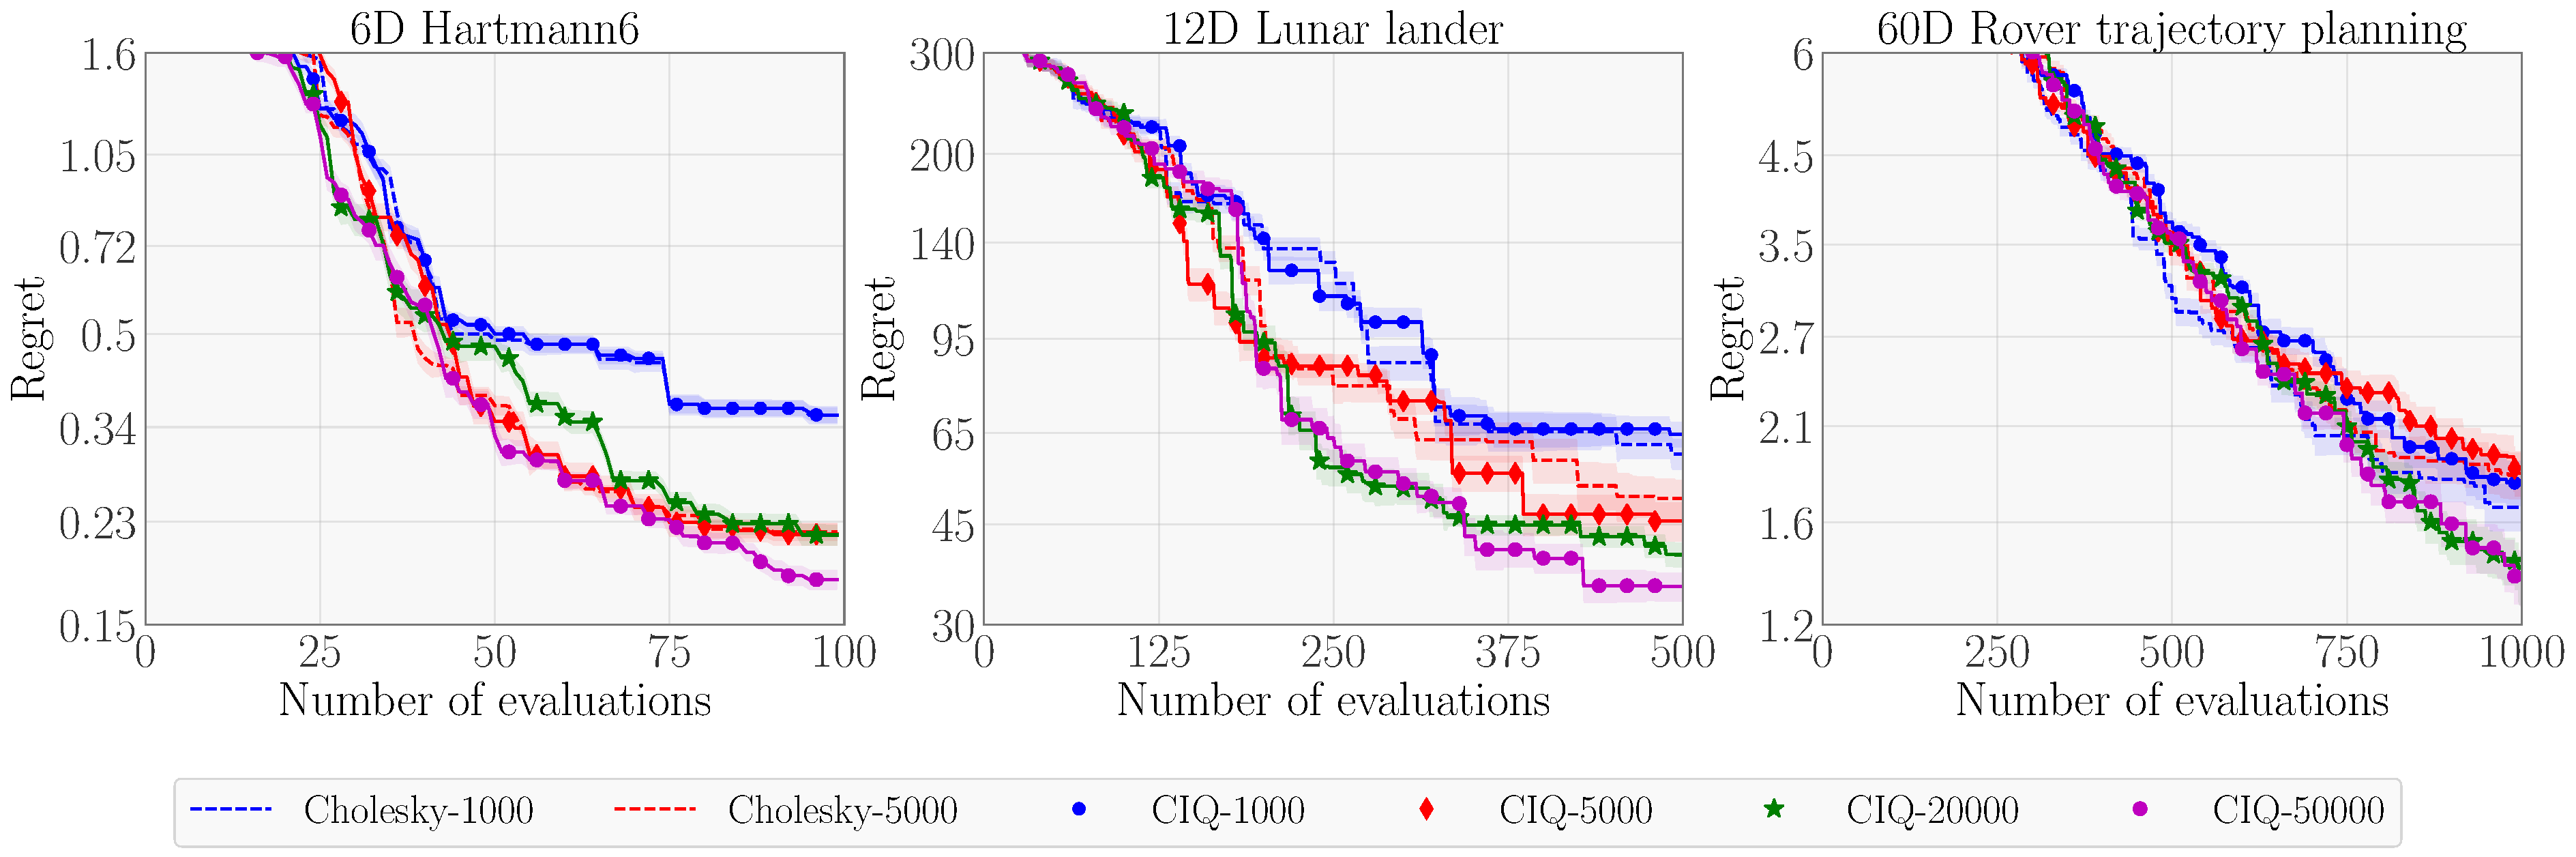
\includegraphics[width=0.85\linewidth]{figures/bo_ciq.pdf}
  \caption[
    A comparison of sampling methods for Bayesian optimization (BO) via TS and \texttt{TuRBO}.
    TS is applied to the Hartmann ($D=6$) and Lunar Lander ($D=12$) while \texttt{TuRBO} is used for Rover ($D=60$).
  ]{
    A comparison of sampling methods for BO.
    BO is applied to the ({\bf left}) Hartmann ($D=6$), ({\bf middle}) Lunar Lander ($D=12$), and ({\bf right}) Rover ($D=60$) problems.
    Methods: Cholesky-$\langle T \rangle$ draws posterior samples with Cholesky at $T$ candidate points.
    CIQ-$\langle T \rangle$ draws posterior samples with CIQ.
    Larger $T$ results in better optimization.
    CIQ enables scaling to $T\geq50,\!000$.
    Each plots shows median regret with one standard deviation in log-scale.
  }
  \label{fig:bayesopt}
\end{figure}

We perform BO using TS on the classical test function ({\bf Hartmann}, $D=6$) and a reinforcement controller tuning problem ({\bf Lunar Lander}, $D=12$) \cite{eriksson2019scalable}.
In addition, we study the high-dimensional BO method \texttt{TuRBO} \cite{eriksson2019scalable} on a rover trajectory planning problem {\bf Rover}, $D=60$) \cite{wang2017batched}.
For each problem we use exact Gaussian processes (no approximations) as the surrogate model and TS as the acquisition function.
Our goal is to determine whether CIQ-based sampling is beneficial by allowing us to accurately scale to larger candidate set sizes.

\paragraph{Baselines.}
With sufficient quadrature points and msMINRES iterations, we can reduce the error of CIQ to machine precision (see \cref{thm:ciq_convergence}).
Therefore, we limit the baseline methods to exact sampling methods, and do not consider stochastic approximations \cite{rahimi2008random} or methods that rely on inducing points \cite{wilson2020efficiently}.
We measure the performance of TS as a function of the candidate set size $T$.
We run TS with $T=1,\!000$, $T=5,\!000$, $T=20,\!000$, and $T=50,\!000$.
We use Cholesky ({\bf TS-Cholesky}) for $T=1,\!000$ and $T=5,\!000$, and CIQ ({\bf TS-CIQ}) for $T=20,\!000$ and $T=50,\!000$.
Note that it would be very challenging and impractical to use Cholesky with $T \geq 10,\!000$, both due to its quadratic memory and its cubic time complexity.

\paragraph{Results.}
We plot the median regret with one standard deviation based on 30 replications in \cref{fig:bayesopt}.
By increasing $T=1,\!000$ to $T=50,\!000$, the final regret is significantly lowered on all problems.
We re-iterate that $T=50,\!000$ is largely impractical with Cholesky sampling methods.
Large candidate sets have previously only been possible with approximate sampling methods.
